\documentclass{endm}
\usepackage{endmmacro}
\usepackage{graphicx}

% The following is enclosed to allow easy detection of differences in
% ascii coding.
% Upper-case    A B C D E F G H I J K L M N O P Q R S T U V W X Y Z
% Lower-case    a b c d e f g h i j k l m n o p q r s t u v w x y z
% Digits        0 1 2 3 4 5 6 7 8 9
% Exclamation   !           Double quote "          Hash (number) #
% Dollar        $           Percent      %          Ampersand     &
% Acute accent  '           Left paren   (          Right paren   )
% Asterisk      *           Plus         +          Comma         ,
% Minus         -           Point        .          Solidus       /
% Colon         :           Semicolon    ;          Less than     <
% Equals        =           Greater than >          Question mark ?
% At            @           Left bracket [          Backslash     \
% Right bracket ]           Circumflex   ^          Underscore    _
% Grave accent  `           Left brace   {          Vertical bar  |
% Right brace   }           Tilde        ~

\newcommand{\Nat}{{\mathbb N}}
\newcommand{\Real}{{\mathbb R}}
\def\lastname{Please list your Lastname here}

\begin{document}

% DO NOT REMOVE: Creates space for Elsevier logo, ScienceDirect logo
% and ENDM logo
\begin{verbatim}\end{verbatim}\vspace{2.5cm}

\begin{frontmatter}

\title{An Article Template}

\author{My Name\thanksref{ALL}\thanksref{myemail}}
\address{My Department\\ My University\\ My City, My Country}

\author{My Co-author\thanksref{coemail}}
\address{My Co-author's Department\\ My Co-author's University\\
   My Co-author's City, My Co-author's Country} \thanks[ALL]{Thanks
   to everyone who should be thanked} \thanks[myemail]{Email:
   \href{mailto:myuserid@mydept.myinst.myedu} {\texttt{\normalshape
   myuserid@mydept.myinst.myedu}}} \thanks[coemail]{Email:
   \href{mailto:couserid@codept.coinst.coedu} {\texttt{\normalshape
   couserid@codept.coinst.coedu}}}

\begin{abstract}
This is a short example to show the basics of using the ENDM style
macro files. Ample examples of how files should look may be found
among the published volumes of the series at the ENDM home page
({\texttt{http://www.elsevier.com/locate/endm}})
\end{abstract}

\begin{keyword}
Please list keywords for your paper here, separated by commas.
\end{keyword}

\end{frontmatter}


\section{Introduction}\label{intro}

This short note provides a guide to using the ENDM macro package for
preparing papers for publication in your conference \emph{Proceedings}.
The \emph{Proceedings} may be printed and hard copies distributed to
participants at the meeting; this is an option conference organizers
may choose to exercise.  The \emph{Proceedings} also will be part of
a volume in the series \emph{Electronic Notes in Discrete Mathematics}
(ENDM), which is published under the auspices of Elsevier B.~V., the
publishers of \emph{Discrete Mathematics} and \emph{Discrete Applied
Mathematics}. The ENDM home page can be found at
\href{http://www.elsevier.com/locate/endm}
{\texttt{http://www.elsevier.com/locate/endm}}

The ENDM macro package consists of two files:
\begin{itemize}
\item \texttt{endm.cls}. This is the basic style file.
\item \texttt{endmmacro.sty}. A macro file containing the definitions
of some of the theorem-like environments and a few other things.
\end{itemize}

The formatting these style files impose should \emph{not} be altered.
The reason for using them is to attain a uniform format for all papers
in the \emph{Proceedings} of which your paper is a part.

Additional macro files can be added using \verb+\usepackage{...}+.
The file \texttt{endmmacro.sty} \emph{must} be included in the
list, as is done at the start of the source file for these
instructions.

The ENDM package requires a relatively up-to-date \LaTeX\ system in
order to be successfully used. This is reflected in two other packages
that are called by endm.cls, which must be available on your machine.
These are:
\begin{itemize}
\item The \texttt{hyperref} package. This package allows the use of
hyperlinks in files prepared using \LaTeX 2e, one of the main features
of Adobe's Acrobat$^{\copyright}$ Reader software. Be sure that you
have at least version 6.69d of this package.
\item The \texttt{ifpdf} package. This is used by hyperref to
differentiate between the use of pdf\LaTeX\ and \LaTeX 2e, followed
by dvips and then ps2pdf.
\end{itemize}

The file \texttt{instraut.pdf} contains information about the use of
\LaTeX to prepare files for online publication by Elsevier. This file
refers to the older version of \LaTeX\ that is no longer suppported,
and that is inadequate for preparing \texttt{.pdf} files for online
publication. Reading this file should answer most of the basic
questions about \LaTeX\ that might arise.


\section{Frontmatter}

The biggest difference between a ``usual'' \LaTeX\ style such as
\texttt{article.sty} and the ENDM package is that the ENDM macro
package requires the title, author's name or names, abstract, keywords
and ``thanks'' all to be included within the \texttt{frontmatter}
environment. At the beginning of the source file for this paper, you'll
notice this. Also, you'll notice that the usual \verb+\maketitle+ is
absent; it no longer is needed. The ENDM style package automatically
generates the title, author's name and address, and related material at
the beginning of the paper. Note also that hyperref has been disabled in
this part of the endm.cls file, so references to footnotes aren't linked
to the appropriate footnotes or addresses. This is an old problem with
\LaTeX, involving the fact that the references within the frontmatter
aren't passed cleanly to the linking software.

For those who have used the ENDM package before, the one new thing to
note is the inclusion of \emph{Keywords} which are now required by
Elsevier.

The ENDM macro package provides two alternatives to listing authors
names and addresses. These are described in detail in the file
\texttt{instraut.pdf}. Basically, listing each author and his or her
address in turn, is the simplest method. But, if there are several
authors and two or more share the same address (but not all authors
are at this address), then the method of listing authors first, and
then the addresses, and of referencing addresses to authors should be
used.

Furthermore, note that an acknowledgment of support (the contents of
\verb+\thanks+) should be done by a separate listing of
\verb+\thanks[NSF]{To the NSF}+ with the optional argument --
\verb+[NSF]+ -- being used for \verb+\thanksref+ which is attached to
those authors acknowledging such support. It is important that the
\verb+\thanks+ not be included within the scope of \verb+\author{}+ or
of \verb+\title{}+, but it must be within the scope of the environment
\texttt{frontmatter}.

More details about added terms such as \verb+\collab+ can be found in
the file \texttt{instraut.pdf} if they are needed.


\section{Sectioning and Environments}

Since ENDM is published through the auspices of Elsevier B.~V., their
style files were used to create the ENDM macro package. Below is a
proof which shows that this package is not much different to most
others:

\begin{definition}
A file is \emph{derived} from another file if it was obtained by making
only a few modifications to the original file.
\end{definition}

\begin{theorem}
The file \texttt{\normalshape endm.cls} is derived from
\texttt{\normalshape elsart.sty}.
\end{theorem}

\begin{proof}
This is clear from the similarity of the output to the output from the
standard Elsevier style files.
\end{proof}

If one wants to start a proof with a descriptive word, such as
``sketch'', then one can use the \verb+\begin{proof*}...\end{proof*}+
environment, as in

\begin{proof*}{Proof (Sketch)}
This can be derived from simple observations.
\end{proof*}

The main difference between the file \texttt{endm.cls} and the
\texttt{elsart.cls} file used for other Elsevier journals is the more
precise format we use. Elsevier's generic style files are meant for
preliminary editing and more precise formatting is imposed using a macro
file designed for the specific Elsevier journal in which the paper will
eventually appear. The \texttt{endm.cls} and \texttt{endmmacro.sty} files
format papers uniformly so that they all are easily recognizable as
belonging to the series \emph{Electronic Notes in Discrete Mathematics}.

All of the usual features of \LaTeX\ are available with these style files.
It is only the formatting that has been rigorously defined. One can use
the sectioning commands \verb+\section,\subsection, \paragraph+
and \verb+\subparagraph.+ The numbering scheme used is one under which
Theorem 1.2.3 is the third numbered item in the second subsection of the
first section of the paper. In order to facilitate cross-references, all
of the named environments given below are numbered and all use the same
numbering scheme.

The file \texttt{endmmacro.sty} contains additional information that is
needed to typeset a paper. It also has the definitions of the $\cal AMS$
\texttt{euler} and \texttt{blackboard bold} fonts builtin. If you want to
use symbols for the natural numbers, the reals, etc., then we prefer that
you use the blackboard bold fonts, and not plain bold fonts. This is
accomplished by using the \verb+\mathbb+ font, as in $\Nat$ or $\Real$.

The names of theorem-like environments are provided in
\texttt{endmmacro.sty}. With the exception of the environment
``Algorithm'', the names of all these are the full name rather than a
shortened version. The environments provided and their names are as
follows:
\begin{itemize}
\item \verb+\begin{theorem} ... \end{theorem}+ for Theorems,
\item \verb+\begin{lemma} ... \end{lemma}+ for Lemmas,
\item \verb+\begin{corollary} ... \end{corollary}+ for Corollaries,
\item \verb+\begin{proposition} ... \end{proposition}+ for Propositions,
\item \verb+\begin{criterion} ... \end{criterion}+ for Criteria,
\item \verb+\begin{alg} ... \end{alg}+ for Algorithms,
\item \verb+\begin{definition} ... \end{definition}+ for Definitions,
\item \verb+\begin{conjecture} ... \end{conjecture}+ for Conjectures,
\item \verb+\begin{example} ... \end{example}+ for Examples,
\item \verb+\begin{problem} ... \end{problem}+ for Problems,
\item \verb+\begin{remark} ... \end{remark}+ for Remarks,
\item \verb+\begin{note} ... \end{note}+ for Notes,
\item \verb+\begin{claim} ... \end{claim}+ for Claims,
\item \verb+\begin{summary} ... \end{summary}+ for Summary,
\item \verb+\begin{case} ... \end{case}+ for Cases, and
\item \verb+\begin{ack} ... \end{ack}+ for Acknowledgements.
\end{itemize}

For example,

\begin{algorithm}[h]
\begin{alg}
Step 1: Write the paper\\
Step 2: Format it with the ENDM macro package\\
Step 3: Ship the whole thing to the Guest Editors\\
\end{alg}
\end{algorithm}


\section{References and Cross-references}

All the cross-referencing facilities of \LaTeX\ are supported, so one
can use \verb+\ref{}+ and \verb+\cite{}+ for cross-references within
the paper and for references to bibliographic items. As is done in this
note, the \emph{References} section can be composed with
\verb+\begin{thebibliography}...\end{thebibliography}+. Alternatively,
Bib\TeX\ can be used to compile the bibliography. Whichever one is used,
the references are to be numbered consecutively, rather than by
author-defined acronyms. Of course you can use your own acronyms for
easy reference to each of the items in the bibliography, as has been
done with the listing for this short note.

Note that the references should \emph{not} be started with a new
\verb+\section+ command.

The package \texttt{hyperref} is automatically loaded by endm.cls and
this makes all the cross-references within the document ``active'' when
the pdf file of the paper is viewed with Adobe's Acrobat$^{\copyright}$
Reader. The format for including a link is simple: simply
insert \verb+\href{URL}+ \verb+{text}+ where \emph{URL} is the URL to
which you want the link to point, and \emph{text} is the text you want
to be highlighted and which will bring up the desired web page when
clicked upon.

\subsection{Particulars about {\normalshape \texttt{.pdf} files}}

We now require that \texttt{.pdf} files be provided for publication
online. A \texttt{.pdf} file is viewable by Adobe's Acrobat$^{\copyright}$
Reader, which can be configured to load automatically within a browser.
Viewing a properly formatted \texttt{.pdf} file with Acrobat$^{\copyright}$
allows the cross-references and links to URLs to be active. In fact,
Elsevier utilizes \texttt{.pdf} files in order to take better advantage
of the web's capabilities.

One point that needs to be emphasized is that you should use Type 1
fonts when you typeset your \LaTeX\ source file. These fonts are
scalable, meaning that they carry information that allows the device
viewing the final output to scale the fonts to suit the viewer being
used (from an onscreen viewer such as Adobe's Acrobat$^{\copyright}$
Reader to printing the file on a printer). You can tell if you have
used the right fonts by viewing the final output on your machine. If
the font looks grainy, then you have not used a Type 1 font. Type 1
fonts can be located at the CTAN archive at
\href{http://www.ctan.org}{\tt http://www.ctan.org}. They are public
domain fonts and do not cost anything when you add them to your system.

Assuming you have Type 1 fonts available, there are several methods
for producing \texttt{.pdf} files.

\paragraph{Using \texttt{dvips} and \texttt{ps2pdf}}

We list this option first since it appears to be the most reliable and
the easiest to use, especially if you include embedded PostScript
graphics (\texttt{.eps} files) in your source file. Simply run \LaTeX
2e on your source file, apply \texttt{dvips} to produce a PostScript
file and then apply \texttt{ps2pdf} to obtain a \texttt{.pdf} file.

\paragraph{The \texttt{DVIPDFM} utility}

Another easy method for producing acceptable \texttt{.pdf} files is
via the utility \texttt{dvipdfm}. This utility is included in
distributions of Mik\TeX, which runs on Windows machines, but it
probably needs to be added to your te\TeX\ distribution, if you are
running \LaTeX\ on a UNIX machine. The utility and precise information
about installing it on your system can be found at the web page
\href{http://gaspra.kettering.edu/dvipdfm/}{\tt
http://gaspra.kettering.edu/dvipdfm/}. In essence, this utility
converts a \texttt{.dvi} file into a \texttt{.pdf} file. So, one can
first prepare the \texttt{.dvi} file using \LaTeX, and then apply the
utility \texttt{dvipdfm} to produce the needed \texttt{.pdf}
file.\footnote{ \emph{Beware}! The utility \texttt{dvipdf} does
\emph{not} produce acceptable \texttt{.pdf} files, and should not be
used. Only \texttt{dvipdfm} should be used to produce \texttt{.pdf}
files.} This utility makes the inclusion of graphics particularly
simple. Those that are included in the \LaTeX\ source file are simply
converted to the \texttt{.pdf} format. As we note below, things are
not so simple with the second alternative, which is to use pdf\LaTeX.

\paragraph{pdf\LaTeX}
An alternative to the first possibilities to produce \texttt{.pdf}
files is to process the source file with pdf\LaTeX. This format is
available from the standard CTAN sites \href{http://www.ctan.org}{\tt
http://www.ctan.org}. It appears that pdf\LaTeX\ and \texttt{hyperref}
have some problems when used together. It is necessary to use
pdf\LaTeX\ version 14d or later in order to minimize these issues. If
your system has an earlier version (most te\TeX\ distributions have
version 13d), then you can update your system by retrieving the latest
version of pdf\LaTeX\ from
\href{ftp://ftp.cstug.cz/pub/tex/local/cstug/thanh/pdftex/}{\tt
ftp://ftp.cstug.cz/pub/tex/local/cstug/thanh/pdftex/}. Even if the
recent versions are used, pdf\LaTeX\ has the same dealing with
references embedded with the \texttt{frontmatter} section described
above for \LaTeX.

But there is one aspect of pdf\LaTeX\ that creates problems. Many
authors include EPS\footnote{EPS stands for \emph{embedded PostScript},
which affords a mechanism for including pre-prepared PostScript files
within a \LaTeX\ document.} files within their papers. While this is
fairly straightforward with \LaTeX, there are a couple of points to
note when attempting this with pdf\LaTeX.

To include a PostScript image in a \texttt{.pdf} file produced with
pdf\LaTeX, you first have to convert the image to a \texttt{.pdf} file.
The conversion can be accomplished most easily using Ghostscript; you
can simply view the file in Ghostview and then print the image to a
\texttt{.pdf} file using the \verb+pdfwriter+ option within Ghostview.
The result for a standard chess board that is part of the Ghostview
distribution is the following image:\\

\begin{center}
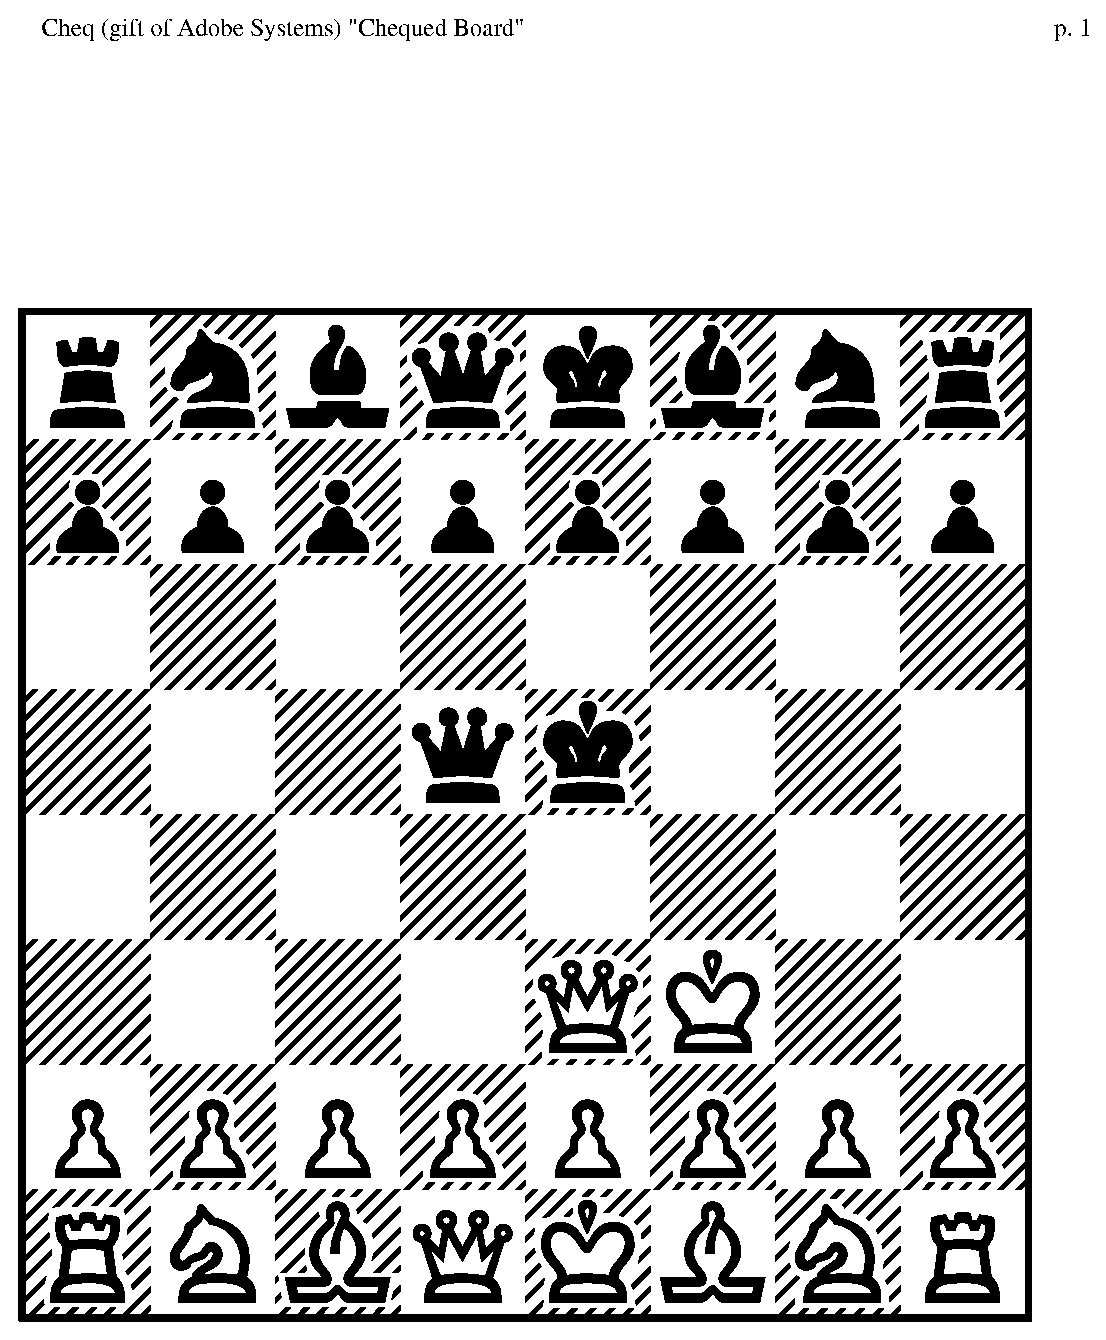
\includegraphics[height=2.8in,width=2.8in]{chess.eps}
\end{center}

Below is a copy of a color image. While pdf\LaTeX\ can handle image
files in other formats, \LaTeX\ can only handle \texttt{.eps} images
reliably.\\

\begin{center}

\includegraphics[height=3.5in,width=3in]{tigre.eps}
\end{center}

\paragraph{Using ENDM Macros with Mac OS X}

Clearly, if your file does not require \texttt{.eps} or other
PostScript files, then you can create the required \texttt{.pdf} file
using any of the standard \TeX\ implementations for the Macintosh. If
you do need to include PostScript files and if you are using \TeX Shop,
then you can specify to use dvips and Ghostview in processing your
file, and then you can apply \texttt{ps2pdf} to create the needed
\texttt{.pdf} file. Alternatively, the Mac OS X operating system is
based on UNIX, so it supports the use of te\TeX\ as described above.


\section{Summary and Remarks}

The ENDM macro package is relatively easy to use and provides a
uniform layout for all the papers that appear in ENDM.

\paragraph{Assigning Volume Numbers}

An additional point worth mentioning is that ENDM has moved to
\emph{ScienceDirect}, Elsevier's main platform for publishing
electronic series. Because \emph{ScienceDirect} cannot easily
accommodate changes to published material, the \emph{Proceedings}
must be entirely ready before they can be published. Volume numbers
will therefore not be assigned for the \emph{Proceedings} until the
final versions of all papers are in.

\paragraph{Copyright Transfer Forms}

Due to the move to \emph{ScienceDirect}, the corresponding author of
each paper published in ENDM must submit a signed Copyright Transfer
Form to Elsevier in order for their paper to be published. A copy of
this form will be sent to each author. Note that the publication of
an abstract or extended abstract in ENDM will not restrict the
author(s) from publishing a full-length article on the same topic and
with the same title in another journal (possibly with another
publisher). Details about the copyright agreement specifying the exact
rights of the authors and the rights of Elsevier are available at
\href{http://authors.elsevier.com/PublisherInfoDetail.html?dc=AGI}
{Elsevier's Author Gateway}.


\section{Bibliographical references}\label{references}

ENDM employs the \texttt{plain} style of bibliographic references in
which references are numbered sequentially and listed in alphabetical
order according to the first author's last name. Please utilize this
style. We have a Bib\TeX\ style file, for those who wish to use it.
It is the file \texttt{endm.bst} which is included in this package.
The basic rules we have employed are the following:
\begin{itemize}
\item Authors' names should be listed in alphabetical order, with the
first author's last name listed first followed by initials or first
name, and with the other authors' names listed as \emph{first name,
last name}.
\item Titles of articles in journals should be in \emph{emphasized}
font.
\item Titles of books, monographs, etc.\ should be in quotations.
\item Journal names should be in plain roman type.
\item Journal volume numbers should be in boldface, immediately
followed by the year of publication enclosed in parentheses in
roman type.
\item References to URLs on the net should be ``active'' and the URL
itself should be in {\tt typewriter} font.
\item Articles should include page numbers.
\end{itemize}

The criteria are illustrated by the examples below.


\begin{thebibliography}{10}\label{bibliography}

\bibitem{cy} Civin, P., and B. Yood, \emph{Involutions on Banach
    algebras}, Pacific J. Math. \textbf{9} (1959), 415--436.
  
\bibitem{cp} Clifford, A. H., and G. B. Preston, ``The Algebraic
  Theory of Semigroups,'' Math. Surveys \textbf{7}, Amer. Math. Soc.,
  Providence, R.I., 1961.
  
\bibitem{f} Freyd, Peter, Peter O'Hearn, John Power, Robert Tennent
  and Makoto Takeyama, \emph{Bireflectivity}, Electronic Notes in
  Theoretical Computer Science {\bf 1} (1995), URL:
  \href{http://www.elsevier.com/locate/entcs/volume1.html}
  {\texttt{http://www.elsevier.com/locate/entcs/volume1.html}}.
  
\bibitem{em2} Easdown, D., and W. D. Munn, \emph{Trace functions on
    inverse semigroup algebras}, U. of Glasgow, Dept. of Math.,
  preprint 93/52.

\bibitem{r} Roscoe, A. W., ``The Theory and Practice of Concurrency,''
  Prentice Hall Series in Computer Science, Prentice Hall Publishers,
  London, New York (1198), 565pp. With associated web site\\  
  \href{http://www.comlab.ox.ac.uk/oucl/publications/books/concurrency/}
  {\texttt{http://www.comlab.ox.ac.uk/oucl/publications/books/concurrency/}}.
  
\bibitem{s} Shehadah, A. A., ``Embedding theorems for semigroups with
  involution, `` Ph.D.  thesis, Purdue University, Indiana, 1982.
  
\bibitem{w} Weyl, H., ``The Classical Groups,'' 2nd Ed., Princeton U.
  Press, Princeton, N.J., 1946.

\end{thebibliography}

\end{document}